\documentclass[aspectratio=169,11pt]{beamer}
\usetheme{default}
\setbeamertemplate{navigation symbols}{}
\setbeamertemplate{footline}{%
  \hfill\insertframenumber/\inserttotalframenumber\hspace*{4pt}\vspace{2pt}%
}
\usepackage{lmodern}
\usepackage[most]{tcolorbox}
\usepackage{listings}
\usepackage{tikz}
\usetikzlibrary{arrows.meta,positioning,shapes.geometric,fit,backgrounds}
\usepackage{booktabs}
\usepackage{hyperref}

\definecolor{lcgreen}{HTML}{2E7D32}
\definecolor{lcblue}{HTML}{1565C0}
\definecolor{lcorange}{HTML}{EF6C00}
\definecolor{lcred}{HTML}{C62828}
\definecolor{codebg}{HTML}{F5F5F5}
\definecolor{docgray}{gray}{0.55}

\newtcolorbox{conceptbox}[1][]{colback=yellow!20,colframe=yellow!60!black,title=#1,fonttitle=\bfseries,top=1pt,bottom=1pt,left=3pt,right=3pt}
\newtcolorbox{warningbox}[1][]{colback=red!15,colframe=red!60!black,title=#1,fonttitle=\bfseries,top=1pt,bottom=1pt,left=3pt,right=3pt}
\newtcolorbox{tipbox}[1][]{colback=green!10,colframe=green!50!black,title=#1,fonttitle=\bfseries,top=1pt,bottom=1pt,left=3pt,right=3pt}
\newtcolorbox{codebox}[1][]{colback=blue!10,colframe=blue!40!black,title=#1,fonttitle=\bfseries,top=1pt,bottom=1pt,left=3pt,right=3pt}

\lstset{
  basicstyle=\ttfamily\tiny,
  backgroundcolor=\color{codebg},
  breaklines=true,
  frame=single,
  rulecolor=\color{blue!40!black},
  keywordstyle=\color{lcblue}\bfseries,
  stringstyle=\color{lcgreen},
  commentstyle=\color{docgray}\itshape,
  language=Python,
  showstringspaces=false,
  tabsize=2,
  xleftmargin=2pt,
  xrightmargin=2pt,
  aboveskip=2pt,
  belowskip=2pt,
}

\newcommand{\docref}[1]{{\scriptsize\color{docgray}[Docs: #1]}}

\title{LangChain v1.2.x: Deep Agents \& Advanced Orchestration}
\subtitle{Building Long-Running, Planning-Capable Agents}
\author{LangChain}
\date{March 2026}

\begin{document}

% ==================== SLIDE 1: TITLE ====================
\frame{\titlepage}

% ==================== SLIDE 2: AGENDA ====================
\begin{frame}[fragile]
\frametitle{Agenda}
\begin{columns}[T]
\column{0.48\textwidth}
\textbf{Part I: Fundamentals}
\begin{enumerate}
    \setlength{\itemsep}{1pt}
  \item Mental Model: What are Deep Agents?
  \item Problems They Solve
  \item Architecture Overview
  \item Core Tools
  \item Building Your First Deep Agent
\end{enumerate}

\column{0.48\textwidth}
\textbf{Part II: Advanced Patterns}
\begin{enumerate}
    \setlength{\itemsep}{1pt}
  \item Long-Running Tasks
  \item Context Management
  \item MCP Integration
  \item Multi-Agent Orchestration
  \item Monitoring \& Fault Tolerance
  \item Comparison Matrix
  \item Pitfalls \& Best Practices
\end{enumerate}
\end{columns}
\vfill
\textcolor{lcblue}{\textbf{45 slides total}} covering v1.2.x (March 2026)
\end{frame}

% ==================== SLIDE 3: MENTAL MODEL ====================
\begin{frame}[fragile]
\frametitle{Mental Model: Deep Agents}

\begin{conceptbox}[What are Deep Agents?]
Autonomous agents capable of:
\begin{itemize}
    \setlength{\itemsep}{1pt}
  \item \textbf{Long-running execution}: tasks that take minutes to hours
  \item \textbf{Multi-step planning}: decompose complex goals into subtasks
  \item \textbf{Persistent state}: offload context to filesystem
  \item \textbf{Sub-agent delegation}: spawn child agents for parallel work
  \item \textbf{Durable execution}: survive interruptions and failures
\end{itemize}
\end{conceptbox}

\vspace{1em}
\begin{center}
\textit{Think of them as mini-employees with planning skills, not just quick chatbot responses.}
\end{center}

\end{frame}

% ==================== SLIDE 4: STANDARD vs DEEP ====================
\begin{frame}[fragile]
\frametitle{Standard Agent vs Deep Agent}

\begin{tabular}{lll}
\toprule
\textbf{Aspect} & \textbf{Standard Agent} & \textbf{Deep Agent} \\
\midrule
Execution Time & Seconds & Minutes to hours \\
Planning & Tool use loop & LLM + task planner \\
State Management & In-memory & Filesystem + DB \\
Task Decomposition & None & Automatic \\
Sub-agent Spawning & No & Yes \\
Fault Recovery & Loss of context & Persistent checkpoints \\
Context Size & Fixed prompt & Offloadable \\
\bottomrule
\end{tabular}

\vspace{1.5em}
\textcolor{lcblue}{\textbf{Key Insight:}} Deep Agents trade speed for sophistication.
\end{frame}

% ==================== SLIDE 5: PROBLEMS SOLVED ====================
\begin{frame}[fragile]
\frametitle{Problems Deep Agents Solve}

\begin{tipbox}[Problem 1: Long-Running Tasks]
Standard agents lose context during multi-minute operations. Deep Agents use persistent storage.
\end{tipbox}

\begin{tipbox}[Problem 2: Context Explosion]
Large research/data tasks overflow token limits. Solution: filesystem offloading.
\end{tipbox}

\begin{tipbox}[Problem 3: Parallel Work]
Can't delegate subtasks to other agents. Solution: sub-agent spawning.
\end{tipbox}

\begin{tipbox}[Problem 4: Fault Tolerance]
Network glitch = start over. Deep Agents recover from checkpoints.
\end{tipbox}

\end{frame}

% ==================== SLIDE 6: ARCHITECTURE ====================
\begin{frame}[fragile]
\frametitle{Deep Agent Architecture}

\begin{center}
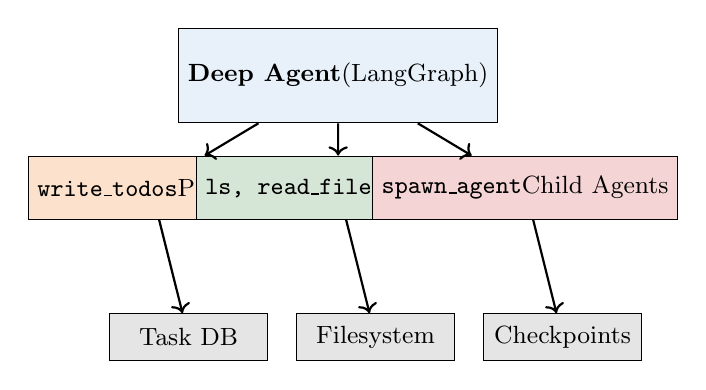
\begin{tikzpicture}[scale=0.95, every node/.style={font=\small}]
  % Main agent box
  \node[draw, rectangle, minimum width=3cm, minimum height=1.2cm, fill=lcblue!10] (agent) at (3,4) {
    \textbf{Deep Agent}\\
    \small(LangGraph)
  };

  % Planning tool
  \node[draw, rectangle, minimum width=2.2cm, minimum height=0.8cm, fill=lcorange!20] (planner) at (0.5,2.5) {
    \texttt{write\_todos}\\
    \small Planner
  };

  % Filesystem tools
  \node[draw, rectangle, minimum width=2.2cm, minimum height=0.8cm, fill=lcgreen!20] (fstools) at (3,2.5) {
    \texttt{ls, read\_file}\\
    \small FS Tools
  };

  % Sub-agent spawner
  \node[draw, rectangle, minimum width=2.2cm, minimum height=0.8cm, fill=lcred!20] (subagent) at (5.5,2.5) {
    \texttt{spawn\_agent}\\
    \small Child Agents
  };

  % Backends
  \node[draw, rectangle, minimum width=2cm, minimum height=0.6cm, fill=gray!20] (db) at (1,0.5) {
    \small Task DB
  };

  \node[draw, rectangle, minimum width=2cm, minimum height=0.6cm, fill=gray!20] (fs) at (3.5,0.5) {
    \small Filesystem
  };

  \node[draw, rectangle, minimum width=2cm, minimum height=0.6cm, fill=gray!20] (checkpoint) at (6,0.5) {
    \small Checkpoints
  };

  % Arrows
  \draw[->, thick] (agent) -- (planner);
  \draw[->, thick] (agent) -- (fstools);
  \draw[->, thick] (agent) -- (subagent);

  \draw[->, thick] (planner) -- (db);
  \draw[->, thick] (fstools) -- (fs);
  \draw[->, thick] (subagent) -- (checkpoint);
\end{tikzpicture}
\end{center}

\vspace{0.5em}
\docref{langchain-deepagents 0.1.x}

\end{frame}

% ==================== SLIDE 7: write_todos TOOL ====================
\begin{frame}[fragile]
\frametitle{The write\_todos Tool: Task Planning}

\begin{lstlisting}
# Deep Agent creates a TODO list at start
from langchain_deepagents import write_todos

# Agent decides task decomposition
todos = write_todos([
  "Fetch latest market data from API",
  "Analyze price trends for 5 assets",
  "Generate trading signals",
  "Format report and save to disk",
])

# Agent tracks progress and can retry failed tasks
# Built-in retry logic for resilience
\end{lstlisting}

\vspace{1em}
\begin{conceptbox}[Key Features]
\begin{itemize}
    \setlength{\itemsep}{1pt}
  \item Automatic task breakdown from agent reasoning
  \item Progress tracking (pending, in-progress, completed)
  \item Sub-task dependencies and ordering
  \item Retry on failure with exponential backoff
\end{itemize}
\end{conceptbox}

\end{frame}

% ==================== SLIDE 8: FILESYSTEM TOOLS ====================
\begin{frame}[fragile]
\frametitle{Filesystem Tools for Context Management}

\begin{lstlisting}
# Read files (manage large context)
content = agent_tools.read_file("data/research.txt")

# List directory contents
files = agent_tools.ls("data/")

# Write or append to files
agent_tools.write_file(
  "data/analysis.txt",
  "Key finding: XYZ correlation..."
)

# Edit specific lines
agent_tools.edit_file(
  "data/report.md",
  start_line=10,
  end_line=15,
  new_content="Updated section..."
)
\end{lstlisting}

\vspace{0.8em}
\begin{warningbox}[Sandbox Warning]
All file operations are sandboxed to agent's working directory for security.
\end{warningbox}

\end{frame}

% ==================== SLIDE 9: SUB-AGENT SPAWNING ====================
\begin{frame}[fragile]
\frametitle{Sub-Agent Spawning \& Delegation}

\begin{lstlisting}
# Parent agent can spawn child agents
from langchain_deepagents import spawn_child_agent

# Delegate a subtask
result = spawn_child_agent(
  goal="Analyze sentiment in customer reviews",
  context={
    "reviews_file": "data/reviews.txt",
    "output_file": "data/sentiment.json"
  },
  max_iterations=20,
  timeout_seconds=300
)

# Results passed back to parent
parent_agent.write_todos(
  f"Parent: sentiment analysis = {result.summary}"
)
\end{lstlisting}

\begin{tipbox}[Benefits]
\begin{itemize}
    \setlength{\itemsep}{1pt}
  \item \textbf{Parallelization}: multiple child agents work simultaneously
  \item \textbf{Isolation}: each child has separate state
  \item \textbf{Scalability}: handle larger problems
\end{itemize}
\end{tipbox}

\end{frame}

% ==================== SLIDE 10: BUILDING A DEEP AGENT ====================
\begin{frame}[fragile]
\frametitle{Building Your First Deep Agent}

\begin{lstlisting}
from langchain import ChatOpenAI
from langchain_deepagents import DeepAgent
from langchain.tools import tool

# Define custom tools
@tool
def fetch_data(source: str) -> str:
  """Fetch data from source."""
  return f"Data from {source}"

# Create agent
llm = ChatOpenAI(model="gpt-4", temperature=0)
agent = DeepAgent(
  llm=llm,
  tools=[fetch_data],
  system_prompt="You are a data analysis agent...",
  max_iterations=30,
  checkpoint_dir="./checkpoints"
)

# Run for long task
result = agent.run(
  goal="Analyze Q1 sales data and forecast Q2"
)
\end{lstlisting}

\docref{DeepAgent docs}

\end{frame}

% ==================== SLIDE 11: DEEP AGENT EXECUTION FLOW ====================
\begin{frame}[fragile]
\frametitle{Deep Agent Execution Flow}

\begin{enumerate}
    \setlength{\itemsep}{1pt}
  \item \textbf{Initialize}: Create agent with LLM + tools
  \item \textbf{Plan}: Call LLM to decompose goal into subtasks
  \item \textbf{Store Plan}: Save todos to database/filesystem
  \item \textbf{Execute Loop}:
  \begin{itemize}
    \setlength{\itemsep}{1pt}
    \item Fetch next pending task
    \item Call tools to complete task
    \item Save results and state
    \item Mark task complete or retry
  \end{itemize}
  \item \textbf{Handle Failures}: If task fails, agent attempts recovery
  \item \textbf{Report}: Final summary saved to file
\end{enumerate}

\vspace{1em}
\begin{center}
\textcolor{lcblue}{\textbf{All state is persistent.}} Network failure $\neq$ data loss.
\end{center}

\end{frame}

% ==================== SLIDE 12: TikZ ARCHITECTURE DIAGRAM ====================
\begin{frame}[fragile]
\frametitle{Deep Agent Execution Architecture}
\vspace{-0.15cm}
\begin{center}
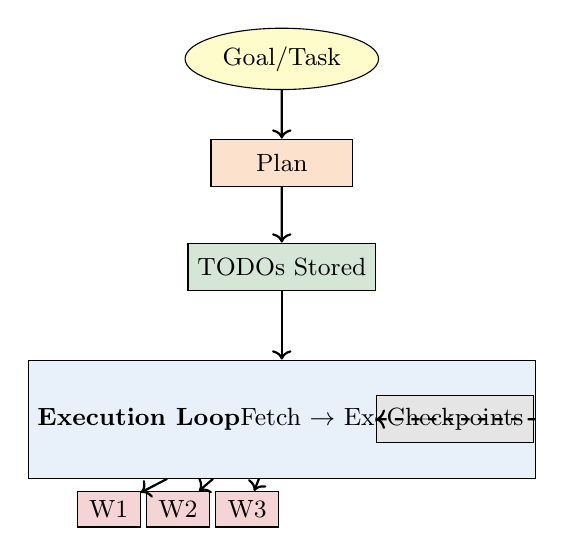
\begin{tikzpicture}[scale=0.88, every node/.style={font=\small}]
  % Goal
  \node[draw, ellipse, fill=yellow!20] (goal) at (3,7) {Goal/Task};

  % Planning phase
  \node[draw, rectangle, fill=lcorange!20, minimum width=1.8cm, minimum height=0.6cm] (planning) at (3,5.5) {Plan};
  \draw[->, thick] (goal) -- (planning);

  % TODO storage
  \node[draw, rectangle, fill=lcgreen!20, minimum width=1.8cm, minimum height=0.6cm] (todos) at (3,4) {TODOs Stored};
  \draw[->, thick] (planning) -- (todos);

  % Execution loop
  \node[draw, rectangle, minimum width=3cm, minimum height=1.5cm, fill=lcblue!10] (loop) at (3,1.8) {
    \textbf{Execution Loop}\\
    \small Fetch $\to$ Execute $\to$ Save
  };
  \draw[->, thick] (todos) -- (loop);

  % Parallel workers
  \node[draw, rectangle, fill=lcred!20, minimum width=0.8cm] (w1) at (0.5,0.5) {W1};
  \node[draw, rectangle, fill=lcred!20, minimum width=0.8cm] (w2) at (1.5,0.5) {W2};
  \node[draw, rectangle, fill=lcred!20, minimum width=0.8cm] (w3) at (2.5,0.5) {W3};

  \draw[->, thick] (loop) -- (w1);
  \draw[->, thick] (loop) -- (w2);
  \draw[->, thick] (loop) -- (w3);

  % Checkpoint
  \node[draw, rectangle, fill=gray!20, minimum width=2cm, minimum height=0.6cm] (ckpt) at (5.5,1.8) {Checkpoints};
  \draw[->, thick, dashed] (loop) -- (ckpt);
\end{tikzpicture}
\end{center}

\textbf{Key:} Multiple workers (sub-agents) execute in parallel. Checkpoints enable resumption.

\end{frame}

% ==================== SLIDE 13: LONG-RUNNING PATTERNS ====================
\begin{frame}[fragile]
\frametitle{Long-Running Task Patterns}

\begin{conceptbox}[Pattern 1: Batch Processing]
\begin{lstlisting}
# Process 1000 items in batches
for batch in batches_of(items, size=100):
  results = agent.process_batch(batch)
  agent.save_checkpoint()  # Persist every batch
\end{lstlisting}
\end{conceptbox}

\begin{conceptbox}[Pattern 2: Periodic Reporting]
\begin{lstlisting}
# Long task with status updates every 5 min
while not agent.is_complete():
  agent.run_step()
  if time_elapsed % 300 == 0:
    agent.write_report("data/status.txt")
\end{lstlisting}
\end{conceptbox}

\begin{tipbox}[Timeout Handling]
Always set \texttt{timeout\_seconds} to prevent runaway agents.
\end{tipbox}

\end{frame}

% ==================== SLIDE 14: CONTEXT MANAGEMENT ====================
\begin{frame}[fragile]
\frametitle{Managing Large Context: Offloading to Filesystem}

\begin{lstlisting}
# Instead of passing giant data in prompt
# Save to file and reference it
agent.write_file("data/dataset.json", large_data)

# In tools, reference the file
@tool
def analyze_data() -> str:
  """Analyze data from file."""
  data = agent.read_file("data/dataset.json")
  # Process data
  return "Analysis complete"

# Agent dynamically reads files as needed
# Keeps prompt tokens manageable
\end{lstlisting}

\vspace{0.8em}
\begin{warningbox}[Prompt Size Limit]
Don't exceed model's context window. Keep per-iteration messages under 10K tokens.
\end{warningbox}

\end{frame}

% ==================== SLIDE 15: MCP INTEGRATION ====================
\begin{frame}[fragile]
\frametitle{MCP (Model Context Protocol) Integration}

\begin{conceptbox}[What is MCP?]
MCP is a standardized protocol for connecting external tools/servers to LLMs.
\end{conceptbox}

\vspace{0.8em}
\begin{lstlisting}
# LangChain integrates MCP servers
from langchain_mcp import MCPClient

# Connect to external MCP server
client = MCPClient(
  server_url="http://localhost:3000",
  server_name="research-tools"
)

# MCP tools auto-available in agent
agent = DeepAgent(
  llm=llm,
  tools=[client.get_tools()],  # MCP tools
)
\end{lstlisting}

\begin{tipbox}[Examples]
MCP servers: web search, database queries, file systems, APIs, code execution.
\end{tipbox}

\end{frame}

% ==================== SLIDE 16: LANGCHAIN-MCP-ADAPTERS ====================
\begin{frame}[fragile]
\frametitle{langchain-mcp-adapters: Auto Tool Conversion}

\begin{lstlisting}
from langchain_mcp_adapters import (
  MCPToolAdapter, PromptMCPAdapter
)

# Automatically wrap MCP resources as tools
adapter = MCPToolAdapter(
  mcp_server_uri="mcp://localhost:3000"
)

# Discovery: find all available tools
tools = adapter.discover_tools()
print(f"Found {len(tools)} MCP tools")

# Create agent with auto-converted tools
agent = DeepAgent(
  llm=llm,
  tools=tools,  # Now LangChain-compatible
)
\end{lstlisting}

\begin{tipbox}[Benefit]
Zero-code integration: any MCP server works automatically.
\end{tipbox}

\docref{langchain-mcp-adapters}

\end{frame}

% ==================== SLIDE 17: MULTI-AGENT ORCHESTRATION ====================
\begin{frame}[fragile]
\frametitle{Multi-Agent Orchestration Patterns}

\begin{conceptbox}[Pattern 1: Supervisor Agent]
One master agent delegates tasks to specialized workers.
\end{conceptbox}

\begin{conceptbox}[Pattern 2: Swarm (Horizontal)]
Multiple agents work in parallel, share results via message bus.
\end{conceptbox}

\begin{conceptbox}[Pattern 3: Hierarchical]
Tree structure: parent spawns children, children spawn grandchildren.
\end{conceptbox}

\begin{center}
\small
\begin{tabular}{lll}
\toprule
\textbf{Pattern} & \textbf{Complexity} & \textbf{Best For} \\
\midrule
Supervisor & Low & Simple delegation \\
Swarm & Medium & Independent parallel tasks \\
Hierarchical & High & Complex decomposition \\
\bottomrule
\end{tabular}
\end{center}

\end{frame}

% ==================== SLIDE 18: SUPERVISOR PATTERN ====================
\begin{frame}[fragile]
\frametitle{Supervisor Pattern Example}

\begin{lstlisting}
from langchain_deepagents import DeepAgent

# Supervisor delegates work
supervisor = DeepAgent(
  llm=llm,
  system_prompt="Delegate tasks to workers..."
)

# Specialized workers
analyst = DeepAgent(
  llm=llm,
  system_prompt="You analyze data..."
)
writer = DeepAgent(
  llm=llm,
  system_prompt="You write reports..."
)

# Supervisor spawns workers for subtasks
supervisor.tools.append(
  spawn_agent(analyst, "Analyze sales data")
)
supervisor.tools.append(
  spawn_agent(writer, "Write report")
)

supervisor.run(goal="Generate quarterly report")
\end{lstlisting}

\end{frame}

% ==================== SLIDE 19: AGENT HANDOFF PATTERNS ====================
\begin{frame}[fragile]
\frametitle{Agent Handoff Patterns}

\begin{lstlisting}
# Agent A detects it can't complete task
# Hands off to Agent B
from langchain.tools import tool

@tool
def handoff_to_specialist(task: str, agent_id: str):
  """Pass control to another agent."""
  # Find agent by ID
  recipient = get_agent(agent_id)
  # Pass context
  result = recipient.run(task)
  return result

# In execution:
# "This needs specialized knowledge" -> handoff
# Original agent pauses, specialist takes over
# Results flow back to original

# Key: all agents share same filesystem
# Easy state sharing between handoffs
\end{lstlisting}

\begin{tipbox}[Use Case]
Multi-stage workflows: collect data → analyze → write → approve.
\end{tipbox}

\end{frame}

% ==================== SLIDE 20: DURABLE EXECUTION ====================
\begin{frame}[fragile]
\frametitle{Durable Execution \& Checkpointing}

\begin{lstlisting}
# Deep Agents auto-checkpoint after each task
agent = DeepAgent(
  llm=llm,
  tools=tools,
  checkpoint_dir="./checkpoints",
  checkpoint_interval=1  # Every task
)

# If interrupted, resume from checkpoint
# Load previous state
result = agent.resume_from_checkpoint(
  checkpoint_id="task-001"
)

# No work is lost!
# Agent knows which tasks are done
# Only retries pending/failed tasks
\end{lstlisting}

\begin{warningbox}[Design]
Checkpoints saved to local filesystem (production: cloud storage recommended).
\end{warningbox}

\docref{Checkpointing Guide}

\end{frame}

% ==================== SLIDE 21: MONITORING DEEP AGENTS ====================
\begin{frame}[fragile]
\frametitle{Monitoring Deep Agent Runs}

\begin{lstlisting}
from langchain_deepagents import AgentMonitor

# Real-time monitoring
monitor = AgentMonitor()

# Track progress
monitor.on_task_start("Fetch data")
monitor.on_tool_call("fetch_api")
monitor.on_task_complete("Fetch data")

# Access metrics
stats = monitor.get_stats()
print(f"Tasks: {stats.completed}/{stats.total}")
print(f"Duration: {stats.elapsed_seconds}s")
print(f"Errors: {stats.error_count}")

# Integration with logging
agent.run(
  goal="...",
  monitors=[monitor]
)

# Export to JSON/CSV
monitor.export_metrics("metrics.json")
\end{lstlisting}

\docref{Monitoring API}

\end{frame}

% ==================== SLIDE 22: COMPARISON MATRIX ====================
\begin{frame}[fragile]
\frametitle{Comparison: Deep Agents vs Alternatives}

\begin{center}
\small
\begin{tabular}{llll}
\toprule
\textbf{Feature} & \textbf{Standard Agent} & \textbf{LangGraph} & \textbf{Deep Agent} \\
\midrule
Speed & ***  & *** & * \\
Long-running & No & ** & *** \\
Planning & No & ** & *** \\
Checkpointing & No & *** & *** \\
Sub-agents & No & ** & *** \\
FS Context Mgmt & No & No & *** \\
Learning curve & Easy & Medium & Medium \\
\bottomrule
\end{tabular}
\end{center}

\vspace{1em}
\begin{tipbox}[Choice Guide]
\begin{itemize}
    \setlength{\itemsep}{1pt}
  \item \textbf{Quick tasks (seconds)}: Standard Agent
  \item \textbf{Complex workflows}: LangGraph
  \item \textbf{Long-running + planning}: Deep Agent
\end{itemize}
\end{tipbox}

\end{frame}

% ==================== SLIDE 23: WHEN TO USE DEEP AGENTS ====================
\begin{frame}[fragile]
\frametitle{When to Use Deep Agents}

\begin{tipbox}[Good Fit]
\begin{itemize}
    \setlength{\itemsep}{1pt}
  \item Research tasks taking 10+ minutes
  \item Data processing with 100+ items
  \item Multi-stage workflows with handoffs
  \item Tasks requiring sub-task delegation
  \item Tasks needing fault tolerance
\end{itemize}
\end{tipbox}

\begin{warningbox}[Poor Fit]
\begin{itemize}
    \setlength{\itemsep}{1pt}
  \item Real-time interactive chat
  \item Tasks under 30 seconds
  \item Simple tool calling
  \item Cost-sensitive applications
\end{itemize}
\end{warningbox}

\vspace{1em}
\begin{center}
\textcolor{lcblue}{\textbf{Key Decision:}} Does your task need planning + resilience?
\end{center}

\end{frame}

% ==================== SLIDE 24: COMMON PITFALLS ====================
\begin{frame}[fragile]
\frametitle{Pitfall 1: Runaway Agents}

\begin{warningbox}[The Problem]
Agent gets stuck in infinite loop or ignores goal completion.
\end{warningbox}

\begin{lstlisting}
# WRONG: No safeguards
agent = DeepAgent(llm=llm, tools=tools)
agent.run(goal="...")  # Could run forever!

# CORRECT: Set limits
agent = DeepAgent(
  llm=llm,
  tools=tools,
  max_iterations=50,      # Hard limit
  timeout_seconds=3600,   # 1 hour max
)
\end{lstlisting}

\begin{tipbox}[Best Practice]
Always set both \texttt{max\_iterations} and \texttt{timeout\_seconds}.
\end{tipbox}

\end{frame}

% ==================== SLIDE 25: PITFALL 2: COST EXPLOSION ====================
\begin{frame}[fragile]
\frametitle{Pitfall 2: Cost Explosion}

\begin{warningbox}[The Problem]
Long-running agents + token-priced LLMs = high costs.
\end{warningbox}

\begin{lstlisting}
from langchain_core.callbacks import TokenUsageCallback
token_tracker = TokenUsageCallback()
agent.run(
  goal="...",
  callbacks=[token_tracker]
)
print(f"Tokens: {token_tracker.total_tokens}")
print(f"Cost: ${token_tracker.estimated_cost}")
\end{lstlisting}

\begin{tipbox}[Mitigation Strategies]
\begin{itemize}
    \setlength{\itemsep}{1pt}
  \item Use cheaper models (Haiku, Opus)
  \item Batch operations to reduce calls
  \item Cache results aggressively
  \item Set \texttt{timeout\_seconds} to prevent waste
\end{itemize}
\end{tipbox}

\end{frame}

% ==================== SLIDE 26: PITFALL 3: CONTEXT OVERFLOW ====================
\begin{frame}[fragile]
\frametitle{Pitfall 3: Context Overflow}

\begin{warningbox}[The Problem]
Accumulating state $\to$ exceeds model's context window.
\end{warningbox}

\begin{lstlisting}
# WRONG: Concatenate everything into prompt
full_context = all_data + all_results + all_logs
agent.run(goal="...", context=full_context)

# CORRECT: Use filesystem
agent.write_file("data/all_results.json", results)
# In tools:
@tool
def summarize():
  """Summarize from file, not prompt."""
  data = agent.read_file("data/all_results.json")
  return summarize(data)
\end{lstlisting}

\begin{tipbox}[Rule of Thumb]
Keep per-iteration context under 4K tokens. Offload the rest.
\end{tipbox}

\end{frame}

% ==================== SLIDE 27: PITFALL 4: POOR ERROR MESSAGES ====================
\begin{frame}[fragile]
\frametitle{Pitfall 4: Unhelpful Error Messages}

\begin{warningbox}[The Problem]
Agent gets cryptic error, doesn't know how to recover.
\end{warningbox}

\begin{lstlisting}
# WRONG: Generic error
@tool
def fetch_data(url: str):
  response = requests.get(url)
  return response.json()

# CORRECT: Helpful recovery
@tool
def fetch_data(url: str):
  try:
    response = requests.get(url, timeout=10)
    return response.json()
  except requests.Timeout:
    return "ERROR: URL unreachable. Try again in 60s."
  except json.JSONDecodeError:
    return "ERROR: Invalid JSON. Check URL format."
\end{lstlisting}

\begin{tipbox}[Best Practice]
Every tool should have clear error messages that guide recovery.
\end{tipbox}

\end{frame}

% ==================== SLIDE 28: TESTING DEEP AGENTS ====================
\begin{frame}[fragile]
\frametitle{Testing Deep Agents}

\begin{lstlisting}
import pytest
from langchain_deepagents import DeepAgent

def test_agent_planning():
  """Test that agent creates reasonable plan."""
  agent = DeepAgent(llm=llm, tools=tools)
  plan = agent.create_plan("Analyze sales")
  assert len(plan.tasks) > 0
  assert all(isinstance(t, Task) for t in plan.tasks)
def test_agent_recovery():
  """Test checkpoint recovery."""
  agent1 = DeepAgent(llm=llm)
  agent1.run_step()
  ckpt_id = agent1.save_checkpoint()
  agent2 = DeepAgent(llm=llm)
  agent2.load_checkpoint(ckpt_id)
  assert agent2.current_task == agent1.current_task
\end{lstlisting}

\begin{tipbox}[Coverage Areas]
\begin{itemize}
    \setlength{\itemsep}{1pt}
  \item Plan generation (reasonable decomposition)
  \item Tool execution (correct results)
  \item Checkpointing (state preservation)
  \item Error recovery (retry logic)
\end{itemize}
\end{tipbox}

\end{frame}

% ==================== SLIDE 29: OBSERVABILITY ====================
\begin{frame}[fragile]
\frametitle{Observability \& Debugging}

\begin{lstlisting}
import logging

# Enable detailed logging
logging.basicConfig(level=logging.DEBUG)

# Structured logging from agent
agent = DeepAgent(
  llm=llm,
  tools=tools,
  verbose=True,  # Log every step
  log_file="agent.log"
)

# In logs you'll see:
# [PLAN] "Analyze data" -> [T1, T2, T3]
# [EXECUTE] T1 "Fetch from API"
# [CALL] tool=fetch_api args={...}
# [RESULT] "200 records retrieved"
# [SAVE] checkpoint-001

# Parse logs for debugging
with open("agent.log") as f:
  for line in f:
    if "[ERROR]" in line:
      print(f"Issue found: {line}")
\end{lstlisting}

\docref{Logging Guide}

\end{frame}

% ==================== SLIDE 30: COST OPTIMIZATION ====================
\begin{frame}[fragile]
\frametitle{Cost Optimization Strategies}

\begin{enumerate}
    \setlength{\itemsep}{1pt}
  \item \textbf{Model Selection}: Use Haiku for planning, Opus for reasoning
  \item \textbf{Batching}: Process multiple items per iteration
  \item \textbf{Caching}: Store tool results, reuse within session
  \item \textbf{Timeouts}: Prevent runaway agents
  \item \textbf{Sampling}: Test on 10% of data first
\end{enumerate}

\vspace{1em}
\begin{lstlisting}
# Example: Use cheaper model for planning
planner_llm = ChatOpenAI(model="gpt-3.5-turbo")
executor_llm = ChatOpenAI(model="gpt-4")

agent = DeepAgent(
  planner_llm=planner_llm,
  executor_llm=executor_llm,
  tools=tools
)
\end{lstlisting}

\vspace{0.5em}
\textcolor{lcblue}{\textbf{Typical 1-hour agent run:}} \$0.50-\$5.00 depending on model choice.

\end{frame}

% ==================== SLIDE 31: PRODUCTION DEPLOYMENT ====================
\begin{frame}[fragile]
\frametitle{Production Deployment Checklist}

\begin{conceptbox}[Before Deployment]
\begin{itemize}
    \setlength{\itemsep}{1pt}
  \item ✓ Set \texttt{max\_iterations} and \texttt{timeout\_seconds}
  \item ✓ Enable checkpointing to cloud storage (S3, GCS)
  \item ✓ Configure logging to centralized system
  \item ✓ Set up alerts for errors/cost spikes
  \item ✓ Test recovery from failures
  \item ✓ Document all custom tools and expected behaviors
  \item ✓ Implement rate limiting on tool calls
  \item ✓ Add monitoring dashboards
\end{itemize}
\end{conceptbox}

\begin{tipbox}[Recommended Stack]
Agent + Cloud Storage + Logging Service + Monitoring = production-ready.
\end{tipbox}

\end{frame}

% ==================== SLIDE 32: REAL-WORLD EXAMPLE: RESEARCH AGENT ====================
\begin{frame}[fragile]
\frametitle{Real-World Example: Research Agent}

\begin{conceptbox}[Goal]
Autonomous agent: investigate a company, write analysis report.
\end{conceptbox}

\begin{lstlisting}
from langchain_deepagents import DeepAgent
from langchain.tools import tool

@tool
def web_search(query: str) -> str:
  """Search web for company info."""
  return results
@tool
def fetch_financials(ticker: str) -> str:
  """Fetch latest financials."""
  return data
agent = DeepAgent(
  llm=ChatOpenAI(model="gpt-4"),
  tools=[web_search, fetch_financials],
  system_prompt="You are a financial analyst. Analyze company metrics, write report.",
  max_iterations=30,
  timeout_seconds=1800
)

result = agent.run(goal="Analyze Apple Inc.")
\end{lstlisting}

\end{frame}

% ==================== SLIDE 33: REAL-WORLD EXAMPLE: DATA PIPELINE ====================
\begin{frame}[fragile]
\frametitle{Real-World Example: Data Processing Pipeline}

\begin{conceptbox}[Goal]
Process 10,000 customer records: clean, enrich, analyze.
\end{conceptbox}

\begin{lstlisting}
# Deep Agent with sub-task delegation
supervisor = DeepAgent(
  llm=llm,
  system_prompt="Manage data processing pipeline"
)
@tool
def spawn_batch_worker(batch_id: int, records):
  """Delegate batch to worker agent."""
  worker = DeepAgent(
    llm=llm,
    system_prompt="Process records batch"
  )
  return worker.run(
    goal=f"Clean and enrich batch {batch_id}",
    context={"records": records}
  )
supervisor.tools.append(spawn_batch_worker)
result = supervisor.run(
  goal="Process all 10k customer records"
)
# Expected: 2-3 hours, auto-checkpoints every batch
\end{lstlisting}

\end{frame}

% ==================== SLIDE 34: LANGCHAIN INTEGRATION RECAP ====================
\begin{frame}[fragile]
\frametitle{How Deep Agents Fit in LangChain Ecosystem}

\begin{center}
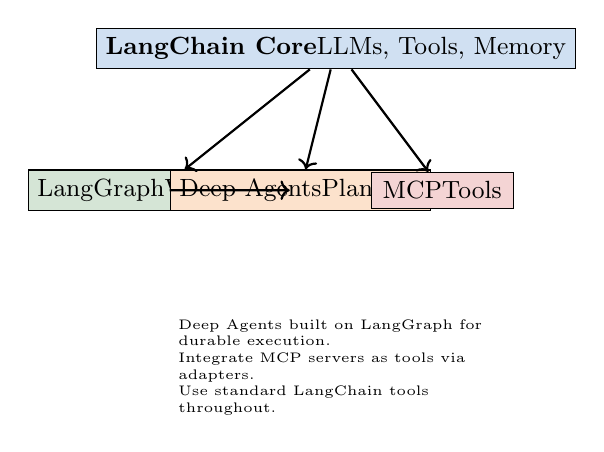
\begin{tikzpicture}[scale=0.9, every node/.style={font=\small}]
  % Core
  \node[draw, rectangle, fill=lcblue!20, minimum width=2cm] (core) at (3,5) {
    \textbf{LangChain Core}\\
    LLMs, Tools, Memory
  };

  % LangGraph
  \node[draw, rectangle, fill=lcgreen!20, minimum width=1.8cm] (langgraph) at (0.5,3) {
    LangGraph\\
    Workflows
  };

  % Deep Agents
  \node[draw, rectangle, fill=lcorange!20, minimum width=1.8cm] (deepagents) at (2.5,3) {
    Deep Agents\\
    Planning
  };

  % MCP
  \node[draw, rectangle, fill=lcred!20, minimum width=1.8cm] (mcp) at (4.5,3) {
    MCP\\
    Tools
  };

  % Arrows
  \draw[->, thick] (core) -- (langgraph);
  \draw[->, thick] (core) -- (deepagents);
  \draw[->, thick] (core) -- (mcp);
  \draw[->, thick] (deepagents) -- (langgraph);

  \node[text width=4cm, font=\tiny] at (3,0.5) {
    Deep Agents built on LangGraph for durable execution.\\
    Integrate MCP servers as tools via adapters.\\
    Use standard LangChain tools throughout.
  };
\end{tikzpicture}
\end{center}

\end{frame}

% ==================== SLIDE 35: SUMMARY & KEY TAKEAWAYS ====================
\begin{frame}[fragile]
\frametitle{Summary: Deep Agents at a Glance}

\begin{conceptbox}[What They Are]
Autonomous, long-running agents with planning, sub-task delegation, and durable execution.
\end{conceptbox}

\begin{conceptbox}[When to Use]
Multi-step research, data processing, complex workflows requiring hours of work.
\end{conceptbox}

\begin{conceptbox}[Core Tools]
\begin{itemize}
    \setlength{\itemsep}{1pt}
  \item \texttt{write\_todos}: Task planning
  \item Filesystem tools: Context management
  \item \texttt{spawn\_agent}: Sub-task delegation
  \item Checkpointing: Fault tolerance
\end{itemize}
\end{conceptbox}

\begin{conceptbox}[Key Benefits]
Persistent state, resilience, parallelization, scalability.
\end{conceptbox}

\end{frame}

% ==================== SLIDE 36: BEST PRACTICES CHEAT SHEET ====================
\begin{frame}[fragile]
\frametitle{Cheat Sheet: Deep Agent Best Practices}

\begin{center}
\small
\begin{tabular}{ll}
\toprule
\textbf{Practice} & \textbf{Guideline} \\
\midrule
Always set limits & \texttt{max\_iterations} + \texttt{timeout\_seconds} \\
Offload large context & Use filesystem, not prompt \\
Monitor costs & Track token usage per run \\
Checkpoint strategy & Enable for any task $>$ 5 minutes \\
Error handling & Provide actionable error messages \\
Testing & Test planning, execution, recovery \\
Logging & Enable verbose logging in production \\
Timeouts & Per-tool + per-agent timeouts \\
\bottomrule
\end{tabular}
\end{center}

\vspace{1em}
\textcolor{lcblue}{\textbf{Remember:}} Deep Agents trade speed for sophistication. Use wisely!

\end{frame}

% ==================== SLIDE 37: SELF-CHECK QUESTIONS ====================
\begin{frame}[fragile]
\frametitle{Self-Check Questions}

\begin{enumerate}
    \setlength{\itemsep}{1pt}
  \item What is the primary difference between a Standard Agent and a Deep Agent?
  \begin{itemize}
    \setlength{\itemsep}{1pt}
    \small
    \item {\color{docgray}Answer: Deep Agents support long-running, planned, resilient execution with sub-task delegation.}
  \end{itemize}

  \vspace{0.5em}
  \item How do Deep Agents prevent context overflow?
  \begin{itemize}
    \setlength{\itemsep}{1pt}
    \small
    \item {\color{docgray}Answer: Filesystem offloading; save large data to files, reference in tools.}
  \end{itemize}

  \vspace{0.5em}
  \item What tool is used for initial task decomposition?
  \begin{itemize}
    \setlength{\itemsep}{1pt}
    \small
    \item {\color{docgray}Answer: \texttt{write\_todos} creates an ordered task list.}
  \end{itemize}

  \vspace{0.5em}
  \item How do you recover from agent interruption?
  \begin{itemize}
    \setlength{\itemsep}{1pt}
    \small
    \item {\color{docgray}Answer: Load from checkpoint; agent resumes from last completed task.}
  \end{itemize}
\end{enumerate}

\end{frame}

% ==================== SLIDE 38: SELF-CHECK QUESTIONS (CONTINUED) ====================
\begin{frame}[fragile]
\frametitle{Self-Check Questions (Continued)}

\begin{enumerate}
    \setlength{\itemsep}{1pt}
  \setcounter{enumi}{4}
  \item Name two sub-agent spawning use cases.
  \begin{itemize}
    \setlength{\itemsep}{1pt}
    \small
    \item {\color{docgray}Answer: Batch processing (10K items), parallel analysis (5 domains).}
  \end{itemize}

  \vspace{0.5em}
  \item What is the Supervisor pattern?
  \begin{itemize}
    \setlength{\itemsep}{1pt}
    \small
    \item {\color{docgray}Answer: One master agent delegates work to specialized worker agents.}
  \end{itemize}

  \vspace{0.5em}
  \item How does MCP integration work in LangChain?
  \begin{itemize}
    \setlength{\itemsep}{1pt}
    \small
    \item {\color{docgray}Answer: Use langchain-mcp-adapters; MCP servers auto-convert to LangChain tools.}
  \end{itemize}

  \vspace{0.5em}
  \item What are the top 3 pitfalls to avoid?
  \begin{itemize}
    \setlength{\itemsep}{1pt}
    \small
    \item {\color{docgray}Answer: Runaway agents (no limits), cost explosion (track tokens), context overflow (offload).}
  \end{itemize}
\end{enumerate}

\end{frame}

% ==================== SLIDE 39: RESOURCES & REFERENCES ====================
\begin{frame}[fragile]
\frametitle{Resources \& References}

\begin{tipbox}[Official Documentation]
\begin{itemize}
    \setlength{\itemsep}{1pt}
  \item LangChain: \url{https://python.langchain.com}
  \item langchain-deepagents: \url{https://github.com/langchain-ai/langchain-deepagents}
  \item LangGraph: \url{https://langchain-ai.github.io/langgraph}
  \item MCP Spec: \url{https://modelcontextprotocol.io}
\end{itemize}
\end{tipbox}

\begin{tipbox}[Recommended Reading]
\begin{itemize}
    \setlength{\itemsep}{1pt}
  \item "Planning and Replanning" (Anthropic, 2024)
  \item "Fault-Tolerant AI" whitepaper
  \item LangGraph Docs: Checkpoint Strategies
\end{itemize}
\end{tipbox}

\end{frame}

% ==================== SLIDE 40: QUICK START TEMPLATE ====================
\begin{frame}[fragile]
\frametitle{Quick Start: Template}

\begin{lstlisting}
from langchain import ChatOpenAI
from langchain_deepagents import DeepAgent
from langchain.tools import tool

@tool
def my_tool(arg: str) -> str:
  """Do something useful."""
  return f"Result: {arg}"

llm = ChatOpenAI(model="gpt-4")
agent = DeepAgent(
  llm=llm,
  tools=[my_tool],
  system_prompt="You help with...",
  max_iterations=30,
  timeout_seconds=3600,
  checkpoint_dir="./checkpoints"
)

result = agent.run(goal="Your task here")
print(result.summary)
\end{lstlisting}

\textcolor{lcblue}{\textbf{Next Step:}} Customize tools, system prompt, and goal for your use case.

\end{frame}

% ==================== SLIDE 41: COMMON EXTENSIONS ====================
\begin{frame}[fragile]
\frametitle{Common Extensions \& Customizations}

\begin{conceptbox}[Extension 1: Custom Tool Wrappers]
Wrap external APIs with Deep Agent semantics (retries, logging).
\end{conceptbox}

\begin{conceptbox}[Extension 2: Multi-Model Delegation]
Route tasks to different models (Haiku for fast, Opus for hard).
\end{conceptbox}

\begin{conceptbox}[Extension 3: External Memory]
Integrate vector DB for semantic search across past results.
\end{conceptbox}

\begin{conceptbox}[Extension 4: Feedback Loops]
Human-in-the-loop: agent asks for approval before risky actions.
\end{conceptbox}

\vspace{0.5em}
\textcolor{lcblue}{\textbf{LangChain Philosophy:}} Composable building blocks. Mix and match!

\end{frame}

% ==================== SLIDE 42: TROUBLESHOOTING GUIDE ====================
\begin{frame}[fragile]
\frametitle{Troubleshooting Common Issues}

\begin{warningbox}[Issue: Agent loops forever]
\textbf{Solution:} Set \texttt{max\_iterations}. Check system prompt clarity.
\end{warningbox}

\begin{warningbox}[Issue: High cost per run]
\textbf{Solution:} Use cheaper model. Enable caching. Batch operations.
\end{warningbox}

\begin{warningbox}[Issue: Agent forgets context]
\textbf{Solution:} Save to filesystem. Use shorter iteration windows.
\end{warningbox}

\begin{warningbox}[Issue: Tool fails, agent error recovery]
\textbf{Solution:} Add detailed error messages. Implement retry logic.
\end{warningbox}

\begin{warningbox}[Issue: Checkpoint loading fails]
\textbf{Solution:} Verify checkpoint file exists. Check permissions.
\end{warningbox}

\end{frame}

% ==================== SLIDE 43: ROADMAP & FUTURE ====================
\begin{frame}[fragile]
\frametitle{Deep Agents Roadmap (2026+)}

\begin{conceptbox}[Q2 2026 Planned]
\begin{itemize}
    \setlength{\itemsep}{1pt}
  \item GPU acceleration for planning
  \item Multi-tenancy support
  \item Web UI for agent monitoring
  \item Advanced scheduling (cron-like)
\end{itemize}
\end{conceptbox}

\begin{conceptbox}[Beyond]
\begin{itemize}
    \setlength{\itemsep}{1pt}
  \item Federated agent networks
  \item Formal verification of plans
  \item Autonomous cost optimization
  \item Self-improving agents
\end{itemize}
\end{conceptbox}

\vspace{1em}
\textcolor{lcblue}{\textbf{Current Status:}} v0.1.x stable, production-ready. Active development.

\end{frame}

% ==================== SLIDE 44: COMMUNITY & SUPPORT ====================
\begin{frame}[fragile]
\frametitle{Community \& Support}

\begin{tipbox}[Getting Help]
\begin{itemize}
    \setlength{\itemsep}{1pt}
  \item \textbf{GitHub Issues}: Report bugs, request features
  \item \textbf{Discord}: Real-time community chat (\url{discord.gg/langchain})
  \item \textbf{GitHub Discussions}: Best practices, architecture Q\&A
  \item \textbf{Stack Overflow}: Tag with \texttt{langchain}
\end{itemize}
\end{tipbox}

\begin{tipbox}[Contributing]
\begin{itemize}
    \setlength{\itemsep}{1pt}
  \item PRs welcome for bugs and features
  \item Docs improvements highly valued
  \item Tool implementations appreciated
\end{itemize}
\end{tipbox}

\vspace{1em}
\textcolor{lcblue}{\textbf{Share your projects!}} Community builds amazing things.

\end{frame}

% ==================== SLIDE 45: CLOSING REMARKS ====================
\begin{frame}[fragile]
\frametitle{Closing Remarks}

\begin{conceptbox}[The Big Picture]
Deep Agents represent a shift toward \textbf{truly autonomous AI systems}:
\begin{itemize}
    \setlength{\itemsep}{1pt}
  \item Not just answering questions
  \item But \textbf{planning}, \textbf{executing}, and \textbf{learning}
  \item Over \textbf{hours}, not milliseconds
  \item With \textbf{resilience} and \textbf{transparency}
\end{itemize}
\end{conceptbox}

\vspace{1em}
\begin{center}
\textcolor{lcblue}{\Large \textbf{The future of AI agents is long-running, resilient, and plan-driven.}}
\end{center}

\vspace{1em}
\begin{center}
\textit{Now go build something amazing with Deep Agents!}
\end{center}

\end{frame}

\end{document}
